\section{Background and Related Work}

\subsection{Intelligent task automation for medical worker capability augmentation}

Similar to the industrial revolution, task automation has been transforming the interaction and collaboration of human workers and AI agents in healthcare, industry, social service and military tasks. This ``white-collar revolution`` has significantly changed the paradigm of human-robot teleoperation. On one hand, intelligent assistive robots augment the physical and cognitive capabilities of human workers, relieve them from repetitive, tedious, effort-demanding, and dangerous tasks. On the other hand, the-state-of-the-art intelligent robot cannot perform complex and risk-sensitive task without human control. As the tasks for robots increasing with the robot capabilities, teleoperation, with more or less task automation, will remain to be the most reliable way to perform the most difficult tasks. It is also the most efficient way to synergize human-robot performance, and explore and utilize robot physical capability.
In this context, physical and cognitive augmentation, in terms of automated information system and automated motion control system,  becomes a necessary components to various medical robotic system. Medical robotic systems have been equipped with various level of intelligent assistance that automate tasks hard or tedious for direct human control. Robot motion planning and learning has enabled the automation the pre-defined motion coordination in rehabilitation and simple, routine surgery procedures.  For more free-style tasks, robot teleoperators have been assisted with motion smoothing and scaling for improved precision control, and with power augmentation in labor-demanding work. However,  due to the little knowledge of task structure and user intent, robots are not clear about which part of the task can be automated and have to depend on teleoperators to micromanage its motion coordination. Conventional interfaces tend to limit the degrees of freedom that human can control directly and/or simultaneously. These interfaces reduce human control efforts, yet impose unnecessary constraints to the motion coordination robot can perform. Novel teleoperation interfaces control map natural human motion using motion capture systems, wearable sensors and exoskeletons, yet the difference in human and robot embodiments usually prevent straightforward motion mapping.  In addition to demanding mental efforts for robot motion control, medical workers can also be limited in or overwhelmed by task information.  Teleoperation interfaces cannot identify the task-relevant perception and performance information, and present in the way comfortable for human to process. The technology limitation compounds the socio-cultural bias in gender, age, and socioeconomic status, prevents the synergy of medical workers and robotic technology.  

\subsection{Prior work in the literature}


Robots have the potential to help distribute expertise around long distances using tele-robotics, to reduce costs by automating routine tasks, and protect workers against occupational hazards and ergonomic strain.  These potential benefits are already being adopted into healthcare.

\textcolor{red}{TODO: need references on gender and age bias with technology.  Needed from Jeanine}

\textcolor{red}{TODO: need references on economic impact of robotics and automation.  Needed from Alex}

\textcolor{red}{TODO: clean up and add references to telerobotics and autonomy}
Collaboration between humans and autonomous robotic agents has the potential to improve safety and efficiency across a wide range of industrial settings, including manufacturing, medicine, maintenance, and construction (Fong, Thorpe, \& Baur, 2001; Tan, Duan, Zhang, Kato, \& Arai, 2009; Kock, et al., 2011; McDonald, Small, Graves, \& Cannon, 1997). An important set of challenges in the design and implementation of human-autonomy collaborative systems is developing a clear understanding of the task environment and potential agent roles, the interdependencies between human and robotic agents, and the impact of disruptions (e.g. (Tan, Duan, Kato, \& Arai, 2010; Hoffman \& Breazeal, 2004; Drury, Scholtz, \& Yanco, 2003; Mutlu, Osman, Forlizzi, Hodgins, \& Kiesler, 2006)).

Managing the safety and efficiency of such systems under dynamic settings is particularly challenging given the complexities of such work environments. For example, a response to a dynamic failure (such as a human or robot breakdown) will have different considerations dependent upon the work architecture (the functional allocation between robots and human) and nature of the work environment (structured vs. unstructured, e.g. (Kolski, Ferguson, Bellino, \& Siegwart, 2006; Scholtz, 2003)). How to effectively optimize safety and efficiency, which are often competing variables, and dynamically reallocate resources accordingly creates a challenging problem for managers and schedulers of such complex systems.

Management of worker and equipment scheduling, coordinating equipment maintenance, tracking of production and safety metrics and ensuring appropriate quality control are all key considerations for supervisors of modern manufacturing environments (e.g. (Brumson, 2008; Brandimarte, 1999)). The challenges associated with managing all of these factors are made more complex by the introduction of collaborative human and robotic work environments, which is a nascent interdisciplinary field. In current manufacturing environments humans and robots work in zones of exclusivity, both physically and for task assignments (Krüger, Lien, \& Verl, 2009; Fryman, 2014; Unhelkar \& Shah, 2015). However, with the emergence of robots that can work alongside humans, like the Baxter™ robot (Figure 1), soon human-robot teams  that jointly work on tasks will be commonplace. 


The increased capabilities that collaborative human-robot teams will bring also introduce complexities in scheduling activities, particularly under dynamic replanning conditions  that occur when both humans and robots “malfunction”, i.e., humans call in sick at the last minute or robots unexpectedly stop working (Wilcox, Nikolaidis, \& Shah, 2013; Stubbs, Wettergreen, \& Hinds, 2007). The impact of these contingencies on the productivity of a manufacturing line will depend upon the nature of the task, the architecture of the work environment, and the availability of substitute workers (either human or robot). The flexibility of the work architecture will dictate the options with which a scheduler or manager can shift assets to minimize the impact on production when problems arise. Indeed, even in current manufacturing operations, such last-minute, dynamic replanning scenarios are difficult to manage even without the added complexity of jointly-tasked human-robot teams (Leitão \& Restivo, 2008). In collaborative human-autonomy environments, addressing such dynamic replanning conditions will be even more challenging, and an inefficient decision could result in a significant decrement in production or increase in safety risk.

There is a long history of research on the incorporation of robotic agents in manufacturing systems (Hägele, Nilsson, \& Pires, 2008; Krüger, Lien, \& Verl, 2009). Typically, these efforts have focused on the use of physical or temporal separation from humans to ensure safety (Marvel \& Bostelman, 2013; Fryman, 2014; Unhelkar \& Shah, 2015; Tan, Duan, Zhang, Kato, \& Arai, 2009; Eilering, Franchi, \& Hauser, 2014). More recently, there has been interest in the inclusion of robotic systems in manufacturing environments that require close interaction and collaboration of human and robotic agents (Office of the Secretary of Defense, 2013; Ryan \& Cummings, 2014; Scanlon, 2009; Rio Tinto, 2014) (Nikolaidis, Ramakrishnan, Gu, \& Shah, 2015). Most of the prior research on human-robot collaboration has focused on the localized methods of interaction and communication of commands and intent between a human worker and a robotic worker (Gombolay, Huang, \& Shah, 2015; Inagaki, Sugie, Aisu, Ono, \& Unemi, 1995; Green, 2008; Bauer, Wollherr, \& Buss, 2008; Fernandez, Balaguer, Blanco, \& Salichs, 2001; Li \& Hauser, 2015; Hoffman, 2013). For example, Fernandez et al. (2001) experimented with determining intent of humans in a collaborative carrying task based on the force signal measured in the arm gripper. Maintaining safety in such collaborative environments has also continued to be an active area of research (Tan \& Arai, 2011; Fryman, 2014; Pedrocchi, Vicentini, Matteo, \& Tosatti, 2013; Matthias, et al., 2011). However, there is very little research on more global interactions of humans and robots in terms of developing integrated schedules, and how such interactions drive large productivity and safety goals.

Traditionally, scheduling of robotic systems have focused on artificial intelligence (AI) or rule-based scheduling (e.g. (Miyashita, 1998; Hall, Kamoun, \& Sriskandarajah, 1998; Sikora \& Shaw, 1997)), though have acknowledged the usefulness of including a human supervisor in the scheduling process (Chen \& Guerrero, 1992). It has been demonstrated that human supervisors can improve scheduling decision-making through the coaching of automated systems, e.g. (Barnes, Chen, Jentsch, \& Redden, 2011; Cummings, Brzezinski, \& Lee, 2007; Adams, 2009; Chen \& Barnes, 2012; Fagerholt, 2004; Törnquist, 2006). While these studies have shown the benefit of automation-aided decision making, these environments generally considered automation in terms of “expert” systems, which operate deterministically by pre-programmed rules. What they have not addressed is the task dependencies and scheduling challenges associated with proposed human-autonomy collaborative manufacturing environments, which contain significant uncertainty and many more stochastic variables.

Still a relatively new field, current research into task scheduling for robotic and collaborative environments focuses on detailed elements of timing and motion constraints (e.g. (Gombolay, Wilcox, \& Shah, 2013; Shah, Conrad, \& Williams, 2009; Boerkoel Jr \& Durfee, 2011; Gowal \& Martinoli, 2012), but does not address higher level considerations such as short and long term impacts to higher level global considerations including overall schedule, throughput, maintenance scheduling, and ergonomic risk. The proposed work aims to fill these gaps by investigating decision-support tools for collaborative manufacturing environments that incorporates both short and long term, and local and global implications of current and proposed schedules.

\subsection{Socio-economic bias in the usage of intelligent medical task automation}

Intelligent task automation aims to improve the availability of high-quality healthcare service while reducing the cost.  It also aims to reduce the control and learning efforts in the usage of healthcare robots, equalize worker performance, lower the barrier to healthcare professions, and improve job satisfaction of medical workers. Despite the good intention of technology development,  the potential psychological and socioeconomic implications needs to be fully understood to evaluate the socioeconomic impacts that may be brought by the usage healthcare robots. 
One issue that needs to be investigated with healthcare robots is the issue of bias.  Bias can come into play in many different forms within health care.  One way in which bias can come into play is through health care workers (i.e., physicians or nurses), Healthcare workers are not immune to bias and use implicit bias related to race, gender, and culture when treating and making decisions about patients (Chapman, Kaatz, \& Carnes, 2013; Taylor, 2003; van Ryn \& Burke, 2000).  Healthcare workers also have preconceived notions of robotic devices and unless they seem easy to use or useful are unlikely to be adopted (BenMessaoud, Kharrazi, \& MacDorman, 2011).  Thus, it is important to understand if assistive robotic technologies can help mitigate this biases or if they will exacerbate them.  
Another way in which bias plays a role in healthcare is through the patients themselves.  Patients experiences with healthcare workers influences their satisfaction with their care, and research has found that female and minority patients are less satisfied with physician and nursing care than male and white patients (Blendon, Scheck, Donelan, et al., 1995; Cooper-Patrick, Gallo, Gonzales, et al., 1999; Foss, 2001; Saha, Komaromy, Koepsell, \& Bindman, 1999).  Minority patients also feel as if they are treated differently and more unfairly than white patients by healthcare workers (Johnson, Saha, Arbelaez, Beach, \& Cooper, 2004).   Thus, it is important to examine how women and minority patients feel about assistive robotic technologies and how they impact their perceptions of the quality of care.  It is possible assistive robotic technologies will be well received as they are receiving high-tech assistance, but it is also possible that assistive robotic technologies will increase feelings of poorer care as it may limit human-to-human interactions between patients and their healthcare providers.  


Another area where bias can come into play is the design of the assistive robotic technologies.  There is already evidence that gender and racial stereotypes emerge in technologies.  For instance, gender stereotypes are often perpetuated in technologies and AI devices because women are often not included in test populations or thought of during the design process (Oost, 2003; Oudshoorn, 2003).  One example of this is that voice recognition systems have a harder time detecting female voices compared to male voices and this included medical voice dictation software (Carty, 2011; Rodger \& Pendharkar, 2004; Taman, 2016).  In addition, women searching for jobs were shown different, and lower paying, search results than men searching for jobs using the same terms (Howard \& Borenstein, 2017).  It is even argued that technological advances help maintain gender biases in society and maintain the status quo (Kilbourne \& Weeks, 1997).  Racial stereotypes are also prevalent in technologies and AI as well (Howard \& Borenstein, 2017).  For instance, Google’s mobile photo app labeled black individuals “gorillas” (Pulliam-Moore, 2015) and image searches for “black teenagers” was more likely to bring up images of criminal activity than a search for “white teenagers” (Howard \& Borenstein, 2017).   Thus, it is important during the design phase of the assistive technologies that measures are taken to ensure the devices limit the proliferation of biases (Howard \& Borenstein, 2017).  

\subsection{Related work of the investigators}

% \begin{wrapfigure}{r}{0.75\linewidth}
\begin{figure}[h!!]
\centering
% \vspace{0.8ex}
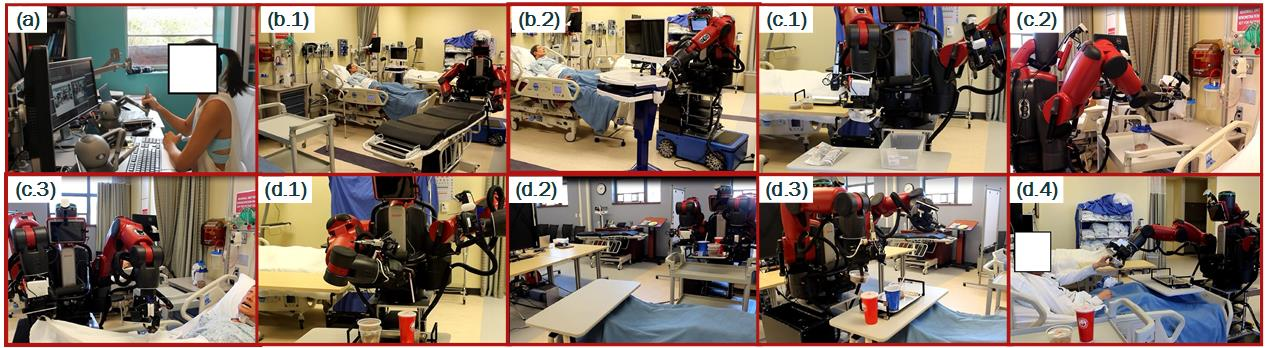
\includegraphics[width=0.99\linewidth]{fig//NursingTask}
\caption{Under (a) direct teleoperation, a mobile humanoid robot tasks can perform complex nursing tasks, including (b.1-2) moving a portable medical devices; (c.1-3) organizing and cleaning the patient's room; and (d.1-4) preparing and serving food to a patient. These tasks involves the coordination among multiple robot components for manipulation, locomotion and active perception.}
\label{NursingTask}
\vspace{1ex}
\end{figure}
% \end{wrapfigure}

\begin{itemize}
\item \textbf{Tele-nursing Robots} In response to the outbreak of highly infectious diseases, including Ebola (2015) and Zika (2016), Tele-Robotic Intelligent Nursing Assistant (TRINA) --- a tele-presence-tele-action mobile humanoid robot system --- has been developed and over frequently performed nursing tasks (see~\fig{NursingTask}). The nursing robot is equipped with fixed cameras mounted at the head and chest, and moving cameras attached to the wrists. Thus, a teleoperator is able to control the coordination of the robot's perception and action arms, in addition to the coordination of different robot components (e.g., arms, hands, mobile base). The experimental system evaluation has demonstrated that on average the tele-nursing robotic system controlled by expert teleoperator is 95X slower than expert human nurse. This performance can be significantly improved by developing a teleoperation interface of more transparent perception and motion mapping. 

\zhi{Figures for tele-surgery tasks to be added}

\item \textbf{Tele-surgical Robots} Surgical procedures are traditionally performed by two or more surgeons along with staff nurses: one serves as the primary surgeon and the other as his/her assistant. Raven IV, a compact multi-arm surgical robotic system, has been developed to enable the collaboration in surgery operation. By automating frequently performed surgical procedures, including dissection, suturing, and tissue manipulation, surgeons can be relieved of the cognitive burden of controlling direct operation and thus focus surgery decision-making. Tele-surgical robot interfaces can further augment a surgeon's cognitive capabilities by integrating ``cloud wisdom'' --- a collaborative decision-making ensemble of multiple intelligence agents, including human experts and AIs. \textcolor{red}{TODO: need details from Jacob.}

% While low-level task automation cognitive augmentation 
% Introducing surgical robots into the operating room has significantly changed the dynamics of interaction between the surgeons and with the surgical site. Through surgical procedure automation, surgical robots relieve the 

% it is  challenging  for  the  surgeon  to  estimate  distances  and
% angles  through  an  endoscope.  Additionally,  with  limited
% vision and/or haptic feedback, extracting the needle from the
% desired  point  often  requires  multiple  attempts,  resulting  in
% increased tissue trauma and extended operation time


% In robot-assisted minimally invasive surgery, a surgeon needs to control the motion of surgical robot arms while adjusting the endoscopic camera to perceive the surgical site. The motion coordination become more complicated when multiple surgical instruments are operating in the shared workspace. The endoscopic camera needs to appropriately with respect to the operating surgical tools, so that the surgeon can intuitively and correctly perceive the spatial relationship at the operation site. The teleoperation interfaces also need to inform the surgeons of their task performance and the patient vital signs, to assist their operation and decision-making.

\item \textbf{Exoskeleton for stroke rehabilitation}
Stroke recovery benefits from intensive and engaged exercises under the direction and assistance of therapists. In stroke rehabilitation, a dual-arm upper limb exoskeleton (e.g., EXO-UL7, see Figure) can assist patient motion during repetitive tasks, provide accurate real-time physical and physiological measurements, promote recovery by coupling the motion of stroke-impacted and healthy arm, and integrate virtual reality games to improve patient engagement and motion-perception coordination. To therapists, the rich measurement information and rehabilitation task prescription parameters cannot be harnessed without cognitive assistance that automates the detection of voluntary motion intent and the evaluation of patient motor performance. Patients also need to be informed of and engaged by feedback on their practice result and performance, to make conscious efforts towards recovery. 

\item \textbf{Hospital administration} The challenges in hospital administration are compounded by significant scheduling uncertainties such as unplanned absences by workers, equipment breakdowns, or worker injuries. The ability of supervisors and management to dynamically adapt role assignments and schedules (what we term as dynamic replanning) is important for dealing with these uncertainties and maintaining adequate patient care. Our prior work has included the preliminary design of a decision support tool for scheduling human shifts in manufacturing environments (Malik, 2013) (Figure 4). This tool allows a supervisor to view the current schedule in the context of required skills and individual ergonomic risk. 

\textcolor{red}{TODO: add prior related work in gender bias, economics, etc.  Needed from Jeanine, Alex}
% \zhi{Figures for tele-rehabilitation tasks to be added}

% \item \textbf{Tele-rehabilitation Robots} Tele-rehabilitation exoskeletons enable therapists to guide and assist remote patients with power augmentation  


\end{itemize}